\section{The Framework}
\label{sec:framework}

\begin{figure}
\centering
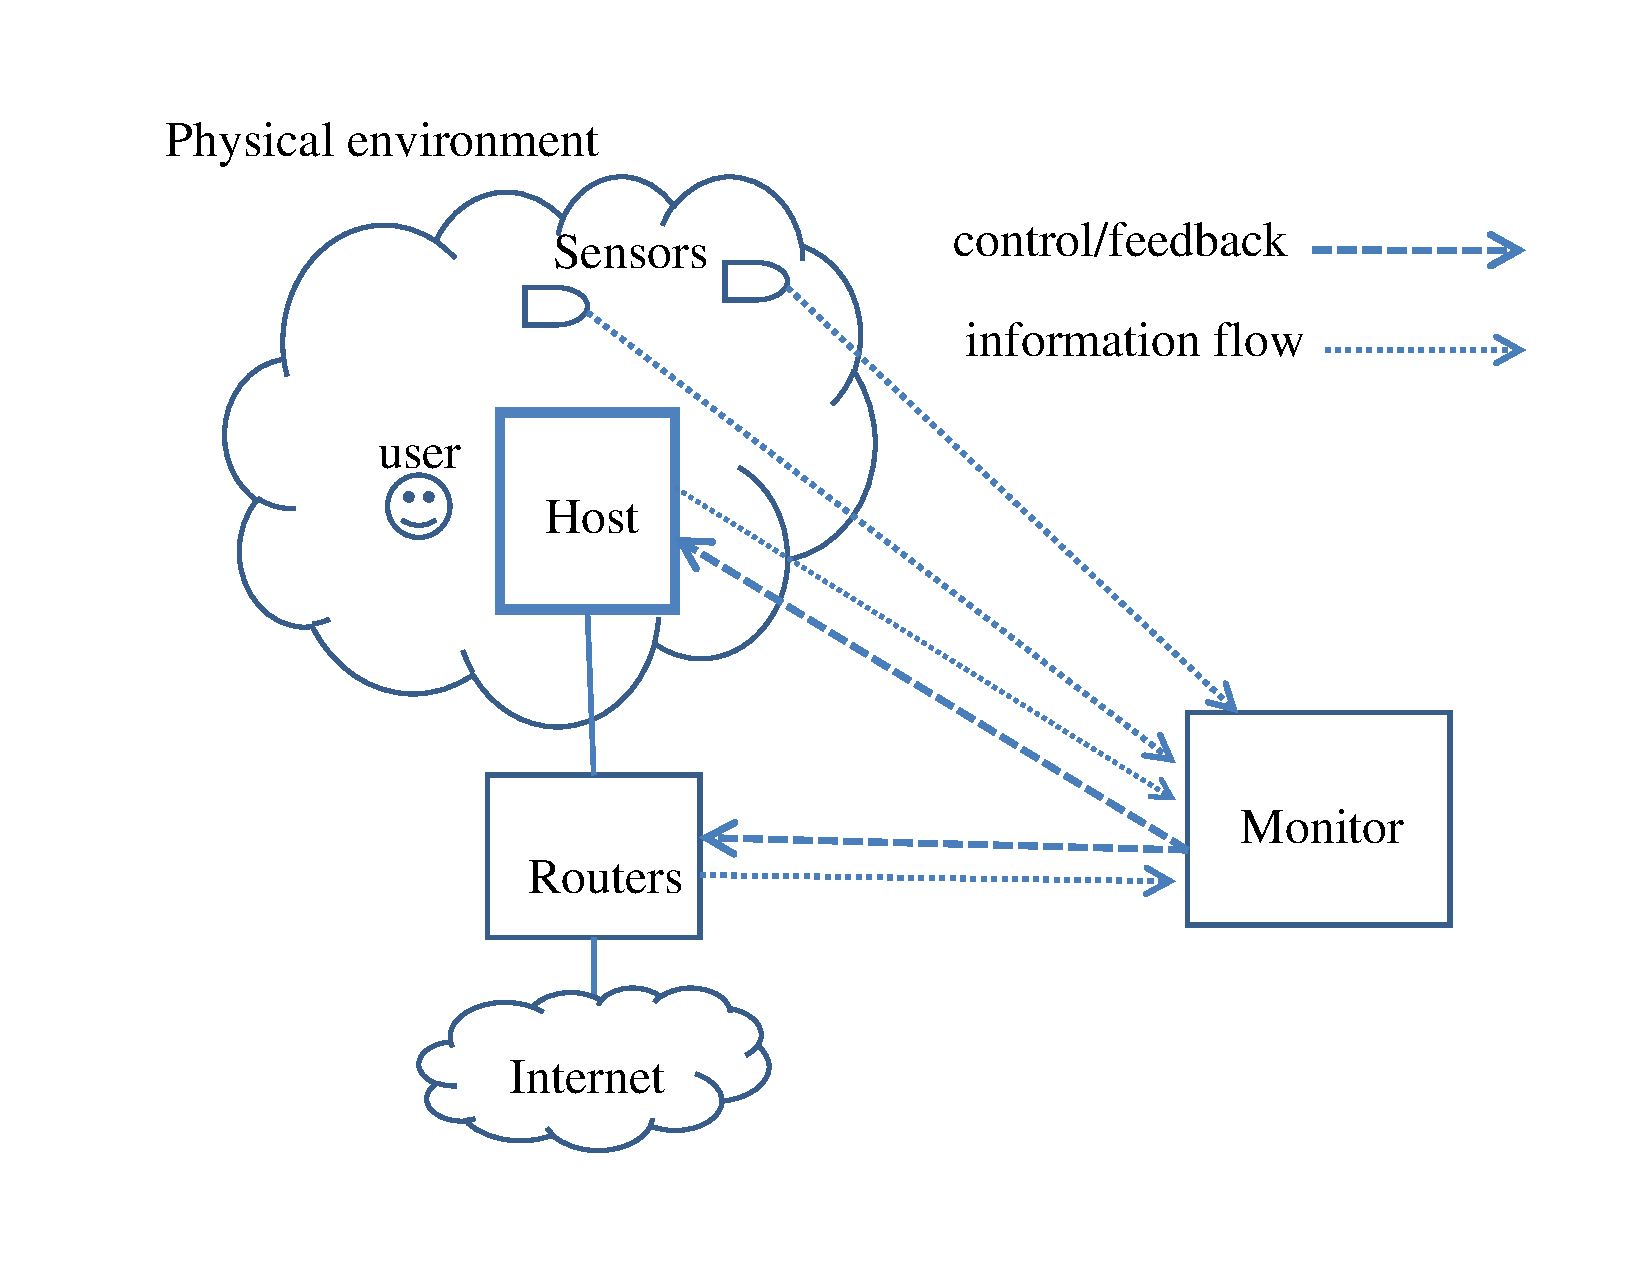
\includegraphics[width=0.95\columnwidth]{sensor/components}
\caption{The components of the framework} \label{fig:components}
\end{figure}

Our framework is composed of the following
entities illustrated in Fig.~\ref{fig:components}:
(i) the host;
(ii) user;
(iii) external environment;
(iv) external sensors;
and (v) external monitor.
In this section, the {\em host} is a stationary computer which typically includes
keyboard, mouse, hard-disk, CPU, monitor, etc., and is operated through 
devices such as keyboard and mouse.

The host, router(s), sensors, monitor and user are situated within
an {\em external environment}.
The host interacts with the external environment through its network
which is controlled by some network {\em routers}.
We assume that all network traffic in and out of the host is
channeled through these routers.
Within the external environment, there are external {\em sensors} for
collecting measurements from the environment and also the host.

{\em Users} in our framework are persons who are
directly accessing the computing resources.
In order for a user to use the host/computing resources, the user
needs to be in the proximity of the host and interacting with it directly
through the keyboard, mouse and display.
We remark that attackers could be accessing the host remotely through
a network connection.
Finally, there is an external {\em monitor} which collects information
collected by the sensors and performs various security functions to
make decisions/control for a security application.

We consider all information processed and stored in the host as {\em
internal} information.
Potentially, internal information
can be manipulated by an adversary if the host is
compromised.
As such, we are more interested in the {\em external} information
as that is immune to tampering by an adversary on the host.
The external information collected by sensors can be varied.
For example, an infra-red sensor can gather information in the
external environment. It could be used to detect whether
a user is sitting in-front of the host's display,
whereas a sensor installed in the router is an example where the sensor
measures data due to host activity.
The three types of information collected by sensors are:
\begin{enumerate}
\item Sensors which measure activity on the host:
A sensor can measure externally resource usage on the host.
The host CPU usage can be measured by using the correlation between
CPU workload which leads to higher power consumption thus causing
increases in the processor temperature.
For example, the temperature can be
measured using a sensor near the motherboard/processor.
As disk drives also make noises when they are used,
a microphone can listen to sounds from the drive; alternatively,
a sensor can measure the disk activity light.

\item Sensors which measure interaction between host and environment:
The main interaction we consider between the host and external environment
is network traffic to/from the router.
The router can itself be utilised as a sensor to measure network traffic
to/from the host.

\item Sensors measuring user presence/activity:
We utilise sensors to detect the presence of a user at the host.
For example, infrared sensors can detect user presence,
alternatively, pressure or motion sensors can be fitted to the user's chair.
A more reliable method to measure user presence is to use
video captured by a camera \cite{biomon,biomon2}.

User activity can also be measured by sensors, e.g.
a pressure sensor to measure keyboard typing.
\end{enumerate}

Although we do not exclude the use of surveillance cameras as the
environment sensors in our framework, the issue of user privacy must
be taken into consideration in an implementation of the framework.
(A recent webcam spying issue highlights the necessity of dealing
with privacy \cite{webcam-spying}).
A microphone not only can detect keyboard activity, but it can also
record conversation among the users. A camera recording the user or
display can also violate workplace privacy policies.
For this reason,
we do not make use of video in our experimental evaluation.
Hence, we mainly consider binary information on user activities, such as
whether a user is present, or detecting keyboard activities.
Such
information can be captured by sensors that are designed or can be converted to give
binary output or other coarse information, which alleviates privacy
concerns, e.g. an infra-red sensor that detects user presence, or a
camera that only outputs the detection outcomes.
There are many commercial wireless multi-sensor
boards which fit our purposes, e.g.
SBT80 from the EasySen
\cite{EasySen} contains a number of sensors including infra-red,
temperature and acoustic.

We remark that privacy may not always be an issue.
In \cite{biomon2}, users found continuous video sent to a monitor to
be an acceptable tradeoff.
We will consider user presence measurements
used for access control in Sec. \ref{sec:app-ac-rate}.

All information gathered is channeled to a
monitor which makes decisions for particular security applications.
The monitor may also have the ability to control
external resources, e.g. control the network traffic at the router.
It could also control some aspects of the host.
%External sensors should communicate to the monitor securely
%to ensure the host is unable to compromise its integrity,
%authenticity and confidentiality.
%One solution is to have a separate private network for the sensors,
%e.g. a wireless sensor network with the external sensors as the nodes.
%A cheaper implementation could tunnel encrypted communication
%through the host but that would be susceptible to DOS attacks if
%the host is compromised.
%The privacy requirements and the need for a separate private
%network fit well with wireless sensor networks equipped with
%multi-modality sensors.
The channel between sensors and monitor should be secure,
e.g. it should be not accessible from the Internet to prevent 
tampering by remote attackers. 
%The model assumes users are cooperative in protecting the host they use, and hence do not tamper with the sensors, the monitor or the communication between them. Scalability is not an issue, such as in an office or lab environment. Each monitor takes care of tens to a few hundreds of hosts. We can assign off-the-shelf PC to be additional monitor to reduce the load of an existing monitor if needed.

Besides wireless sensor networks, many physical security systems
can provide relevant information for our monitor. For
example, the door entry control system
can give information about persons who gain access to
a machine room, while surveillance cameras can
reliably detect the presence of users near a console or other devices
like scanner and printer. Although physical security systems are costly,
an organization could already have such systems in-place,
together with a management system that collects and processes the data.

%It is possible for an attacker to gain information similar to
%the data collected from sensors, if the host is compromised, e.g. CPU
%temperature can be collected by the host and user presence
%can be inferred from keyboard or mouse events.
%Nevertheless,
%the CPU temperature and user presence information collected by sensors
%are still authentic and not subject to tampering.
